\documentclass[a4paper,12pt]{article}
\usepackage[utf8]{inputenc}
\usepackage{graphicx}
\usepackage{fancyhdr}
\usepackage{amsmath}
\usepackage{adjustbox}
\usepackage{mathtools}
\usepackage{float}
\usepackage[spanish, es-nodecimaldot]{babel} 
\usepackage{lastpage}
\usepackage{amssymb} % Para símbolos matemáticos adicionales
\usepackage{hyperref}
\usepackage{cleveref}
%\usepackage[none]{hyphenat}
\usepackage{array}
\usepackage{listings}
\usepackage{xcolor}

\usepackage{multirow}
\usepackage{textcomp}
\usepackage[left=2.5cm, right=2.5cm, top=3cm, bottom=3cm]{geometry}

\lstset{ 
    language=Matlab,                     % El lenguaje del código
    basicstyle=\ttfamily,                % Tipo de letra
    keywordstyle=\color{blue},           % Color para palabras clave
    commentstyle=\color{green!60!black}, % Color para comentarios
    numbers=left,                        % Numeración de las líneas
    numberstyle=\tiny\color{gray},       % Estilo para los números
    stepnumber=1,                        % Mostrar número en cada línea
    tabsize=4,                           % Tamaño de tabulación
    breaklines=true,                     % Partir líneas largas
    showspaces=false,                    % No mostrar los espacios en blanco
    showstringspaces=false,              % No mostrar espacios dentro de strings
    showtabs=false,                      % No mostrar tabs
}

\graphicspath{{Imagenes/}}

% Encabezado y pie de página
\pagestyle{fancy}
\fancyhf{}
\setlength{\headheight}{30 pt}
\renewcommand{\headrulewidth}{0.2pt}
\fancyhead[R]{\begin{tabular}{@{}l@{}}
\includegraphics[scale=0.4]{escudo.PNG}\end{tabular}}
\fancyhead[L]{\begin{tabular}{@{}c@{}} \textbf{Robótica I - Año: 2024} \\ Trabajo Práctico 5: Cinemática Inversa \end{tabular}}


\fancyfoot[R]{\thepage}
\fancyfoot[C]{\begin{tabular}{@{}c@{}}\textbf{BORQUEZ PEREZ Juan Manuel}\\ \textbf{Legajo 13567}\end{tabular}}
\renewcommand{\footrulewidth}{0.2pt}

\begin{document}

\begin{titlepage}
    \centering
    \vspace*{5cm}
    {\Huge\bfseries Informe de Trabajo Práctico N°5B}\\
    \vspace{0.2cm}
    {\Large \textbf{Cinemática Inversa}}\\
    \vspace{0.5cm}
    {\Large Robótica I}\\
    \vspace{0.5 cm}
    {\Large Ingeniería en Mecatrónica}\\
    \vspace{0.2 cm}
    {\Large Facultad de Ingeniería - UNCUYO}\\
    \vspace{1.5cm}
    Alumno: Juan Manuel BORQUEZ PEREZ\\
    Legajo: 13567\\
    \vfill
    {\begin{tabular}{@{}c@{}}
\includegraphics[scale=0.4]{escudo.PNG}\end{tabular}}\hspace{10pt}
    %Año 2023
\end{titlepage}
\section{Robot}
\begin{figure}[H]
    \centering
    \begin{adjustbox}{scale = 0.55, max width=\columnwidth}
        \framebox{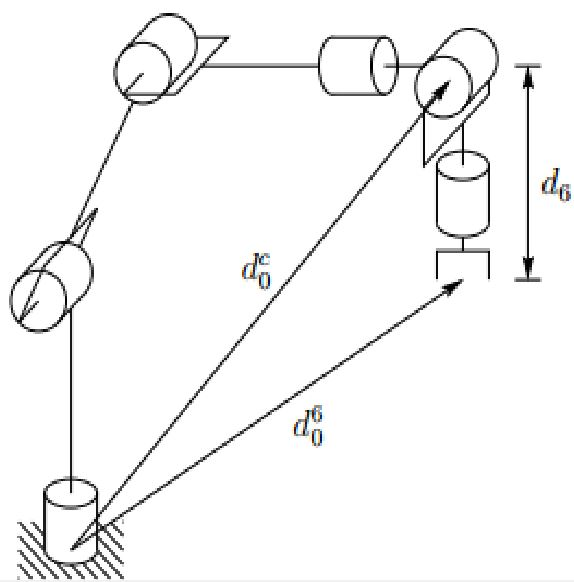
\includegraphics{13-Spong1.JPG}}
    \end{adjustbox}
    \caption{Robot 6gdl - muñeca esférica}
    \label{robot 6gdl}
\end{figure}

La definición de los sistemas en el robot es la que se indica en \cref{sistemas DH}
\begin{figure}[H]
    \centering
    \begin{adjustbox}{scale = 0.55, max width=\columnwidth}
        \framebox{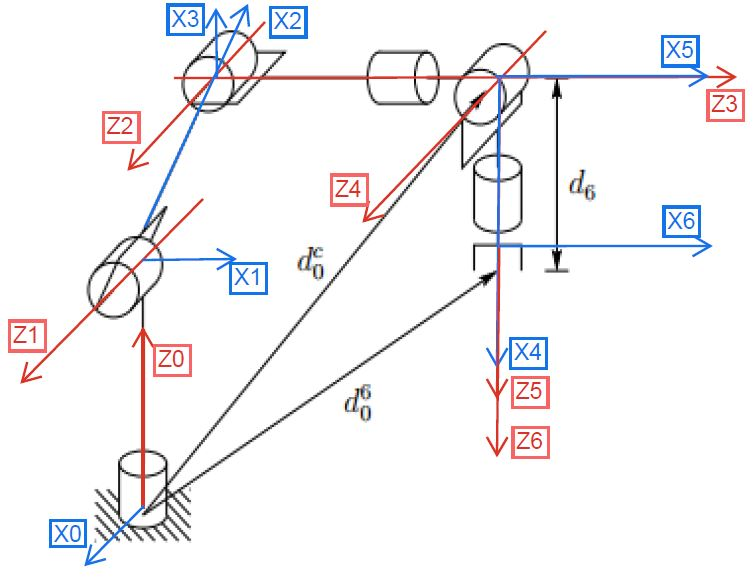
\includegraphics{15-DH_6gdl.JPG}}
    \end{adjustbox}
    \caption{Robot 6gdl - Sistemas DH}
    \label{sistemas DH}
\end{figure}

La matriz de DH que resulta es \cref{matriz DH}. Para el caso, se utilizaran solamente
valores unitarios para los parámetros de longitud de DH ($a_i$ y $d_i$).

\begin{table}[H]
    \centering
    \begin{tabular}{|c|c|c|c|c|c|}
    \hline
    Sistema & $\theta$  & $d$        & $a$    & $\alpha$  & $\sigma$ \\ \hline
    1       & $q_1$     & $d_1$      & $0$    & $\pi/2$   & 0        \\ \hline
    2       & $q_2$     & $0$        & $a_2$  & $0$       & 0        \\ \hline
    3       & $q_3$     & $0$        & $0$    & $\pi/2$   & 0        \\ \hline
    4       & $q_4$     & $d_4$      & $0$    & $\pi/2$   & 0        \\ \hline
    5       & $q_5$     & $0$        & $0$    & $\pi/2$   & 0        \\ \hline
    6       & $q_6$     & $d_6$      & $0$    & $0$       & 0        \\ \hline
    \end{tabular}
    \caption{Robot 6gdl - Matriz DH}
    \label{matriz DH}
\end{table}

\section{Ejercicio 1: Primer Problema de Pieper}
\begin{figure}[H]
    \centering
    \begin{adjustbox}{scale = 0.55, max width=\columnwidth}
        \framebox{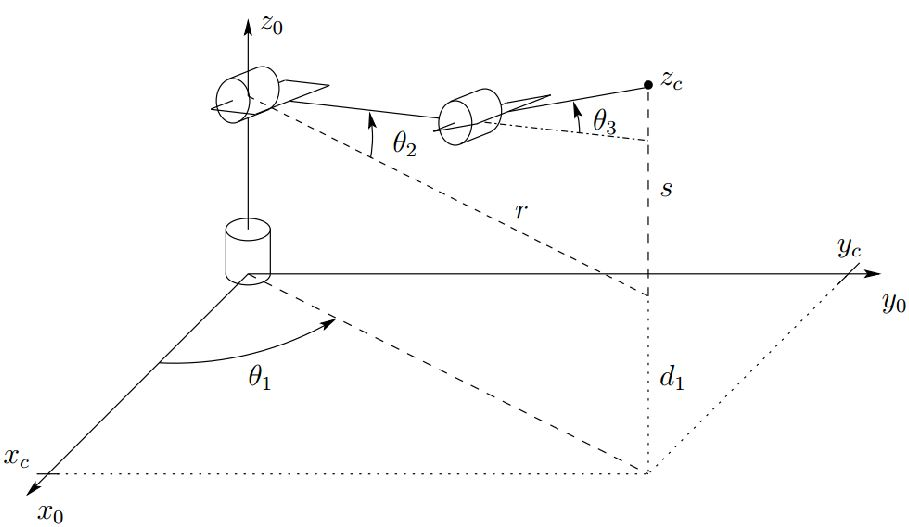
\includegraphics{14-Spong2.JPG}}
    \end{adjustbox}
    \caption{Robot 6gdl - Primer problema de Pieper}
    \label{primer problema pieper}
\end{figure}

Como se puede observar en el esquema cinemático de la \cref{robot 6gdl} los eslabones
1, 2, 3 y 4 se mueven siempre en un mismo plano que contiene al eje $Z_0$ y el ángulo que
el mismo forma con respecto al plano $X_0Z_0$ es el ángulo $\theta_1$. En la \cref{plano q1} se muestra en otra perspectiva
en donde se muestran los dos posibles valores para el ángulo.

\begin{figure}[H]
    \centering
    \begin{adjustbox}{max width=\columnwidth}
        \framebox{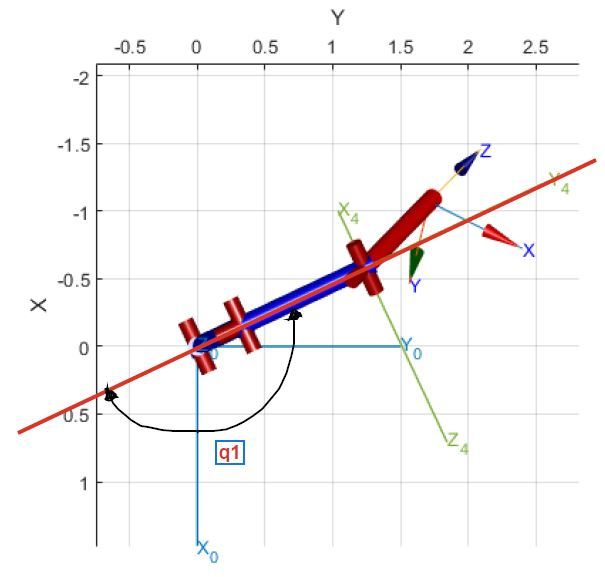
\includegraphics{16-q1.JPG}}
    \end{adjustbox}
    \caption{Plano $q_1$}
    \label{plano q1}
\end{figure}

Luego se obtiene $q_1$ como en la \cref{q1}
\begin{align}
    \begin{cases}
        (q_1)_1 = atan2(y_c, x_c)\\
        (q_1)_1 < 0 \Rightarrow (q_1)_2 = (q_1)_1 + \pi\\
        (q_1)_1 > 0 \Rightarrow (q_1)_2 = (q_1)_1 - \pi\\
    \end{cases}
    \label{q1}
\end{align}

Para cada valor de $q_1$ se tiene la transformación
$\prescript{0}{}{T_1}$ y con la misma se obtiene $\prescript{1}{}{\overline{p_c}}$ como
$\prescript{1}{}{\overline{p}_c} = \left(\prescript{0}{}{T_1}\right)^{-1}\prescript{0}{}{\overline{p}_c}$.
El problema queda entonces formulado como se muestra en \cref{q23}. Se puede ver que  
es equivalente al de la cinemática inversa de un robot RR planar que se vió en la ``parte A'' de este trabajo, como 
queda denotado por los eslabones pintados en negro y las articulaciones con círculos rojos. Para completar la analogía con un RR planar, en la figura se define un sistema 
auxiliar $S3^{\prime}$ junto con la variable $q_3^{\prime}$. La longitud del primer y segundo eslabón en el RR planar son $a_2$ y $d_4$ del robot respectivamente.

Luego, $q_2$ y $q_3^{\prime}$ se obtienen siguiendo el procedimiento para el RR planar. Finalmente se usa la \cref{q3 q3prima} para obtener $q_3$.

\begin{figure}[H]
    \centering
    \begin{adjustbox}{max width=\columnwidth}
        \framebox{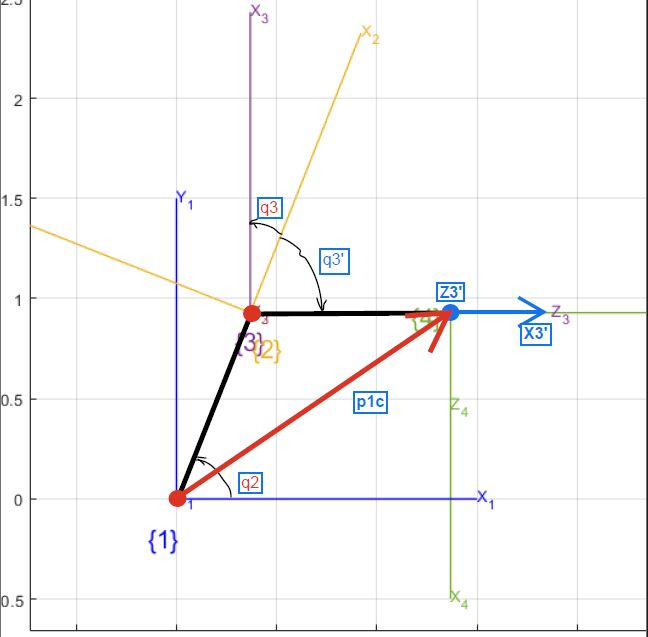
\includegraphics{17-q2.JPG}}
    \end{adjustbox}
    \caption{Plano $q_{23}$}
    \label{q23}
\end{figure}

\begin{equation}
    q_3= \frac{\pi}{2} - q_3^{\prime}
    \label{q3 q3prima}
\end{equation}

\section{Ejercicio 2: Segundo Problema de Pieper}
Dado que se conocen los valores de $q_1$, $q_2$ y $q_3$ se obtiene 
$\prescript{0}{}{T_3}$ (para cada terna). Con esta, se determina $\prescript{3}{}{T_6}$ 
como $\prescript{3}{}{T_6} = \prescript{0}{}{T_3}^{-1}\prescript{0}{}{T_6}$.

El problema hasta aquí queda formulado gráficamente como se indica en \cref{plano q4}.
Se puede observar en \cref{sistemas DH} que el $Z_6$ siempre se mueve en el plano determinado por
$Z_3$ y $X_4$, de manera que su proyección en el plano $X_3Y_3$ coincide que la de $X_4$ sobre el mismo plano.
Así, se puede determinar $q_4$ como el ángulo entre el $Z_3X_4$ (señallado en negro en la figura) y el eje $X_3$, existiendo
los dos posibles valores indicados en la figura.

\begin{figure}[H]
    \centering
    \begin{adjustbox}{max width=\columnwidth}
        \framebox{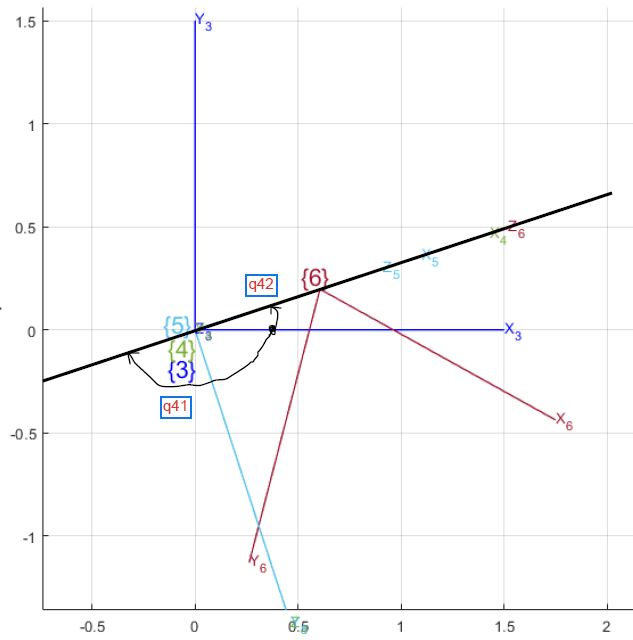
\includegraphics{18-q4.JPG}}
    \end{adjustbox}
    \caption{Plano $q_{4}$}
    \label{plano q4}
\end{figure}

Sean $\prescript{3}{}{n_6}$, $\prescript{3}{}{o_6}$ y $\prescript{3}{}{a_6}$ los 
versores del sistema dado por $\prescript{3}{}{T_6}$. El $\prescript{3}{}{a_6}$ da la dirección de $Z_6$. Luego se determina
$q_4$ a partir de sus componentes 1 y 2 como:

\begin{align}
    \begin{cases}
        (q_4)_1 = atan2\left(\left(\prescript{3}{}{a_6}\right)_2, \left(\prescript{3}{}{a_6}\right)_1\right)\\
        (q_4)_1 < 0 \Rightarrow (q_4)_2 = (q_4)_1 + \pi\\
        (q_4)_1 > 0 \Rightarrow (q_4)_2 = (q_4)_1 - \pi\\
    \end{cases}
    \label{q4}
\end{align}

Obtenido $q_4$, se determina ahora $\prescript{4}{}{T_6}$ como $\prescript{4}{}{T_6} = \prescript{3}{}{T_4}^{-1}\prescript{3}{}{T_6}$ y el problema
queda como se indica en \cref{plano q5}. Luego se obtiene 

\begin{align}
    \begin{cases}
        \alpha = atan2\left(\left(\prescript{4}{}{a_6}\right)_2, \left(\prescript{4}{}{a_6}\right)_1\right)\\
        q_5    = \frac{\pi}{2} + \alpha
    \end{cases}
    \label{q5}
\end{align}

\begin{figure}[H]
    \centering
    \begin{adjustbox}{max width=\columnwidth}
        \framebox{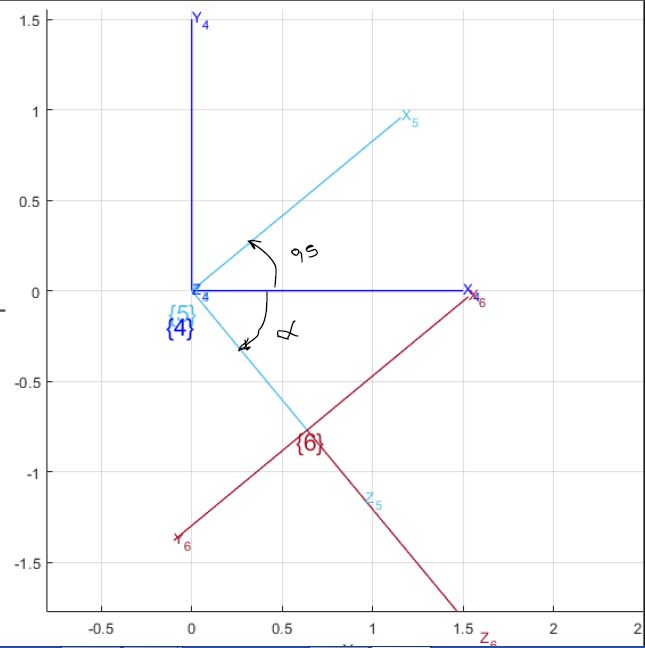
\includegraphics{19-q5.JPG}}
    \end{adjustbox}
    \caption{Plano $q_{5}$}
    \label{plano q5}
\end{figure}

Finalmente se obtiene $\prescript{5}{}{T_6}$ como $\prescript{5}{}{T_6} = \prescript{4}{}{T_5}^{-1}\prescript{4}{}{T_6}$ y el problema
queda como en \cref{plano q6}. De donde se obtiene facilmente:

\begin{align}
    q_6 = atan2\left(\left(\prescript{5}{}{n_6}\right)_2, \left(\prescript{5}{}{n_6}\right)_1\right)\\
    \label{q6}
\end{align}

\begin{figure}[H]
    \centering
    \begin{adjustbox}{max width=\columnwidth}
        \framebox{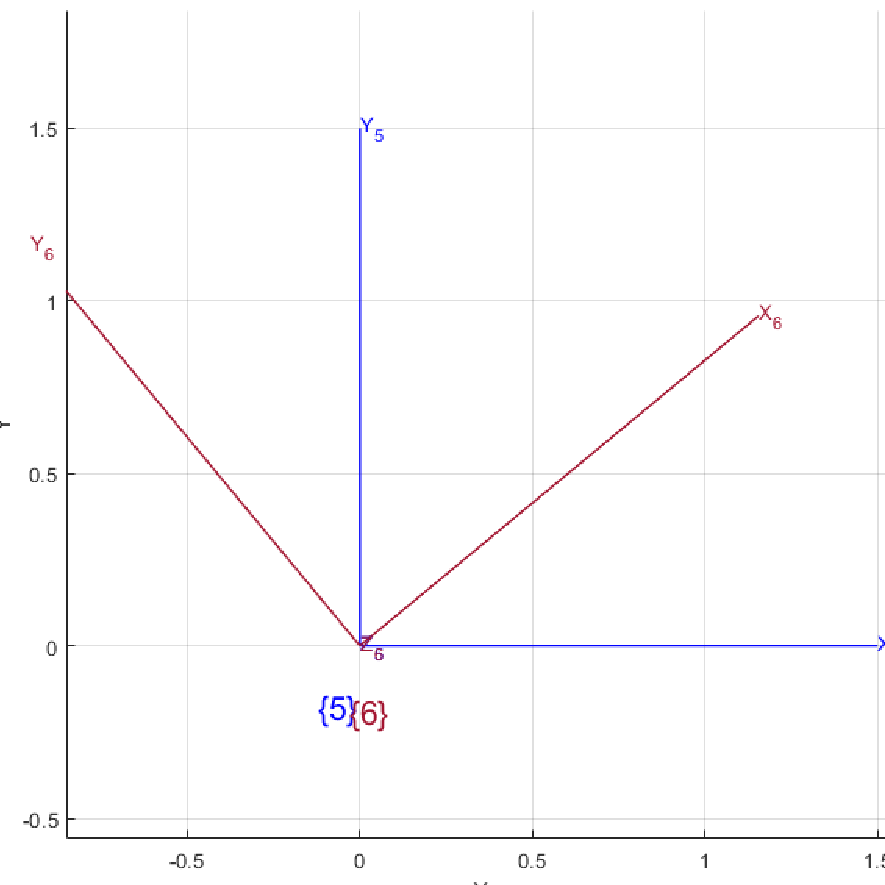
\includegraphics{20-q6.pdf}}
    \end{adjustbox}
    \caption{Plano $q_{6}$}
    \label{plano q6}
\end{figure}




%\begin{equation*}
%    \prescript{O}{}{Rot_M} = 
%    \begin{bmatrix}
%        0.500 & -0.866\\
%        0.866 & 0.500
%    \end{bmatrix}
%\end{equation*}

%\begin{figure}[H]
%    \centering
%    \begin{adjustbox}{scale = 0.85, max width=\columnwidth}
%        \framebox{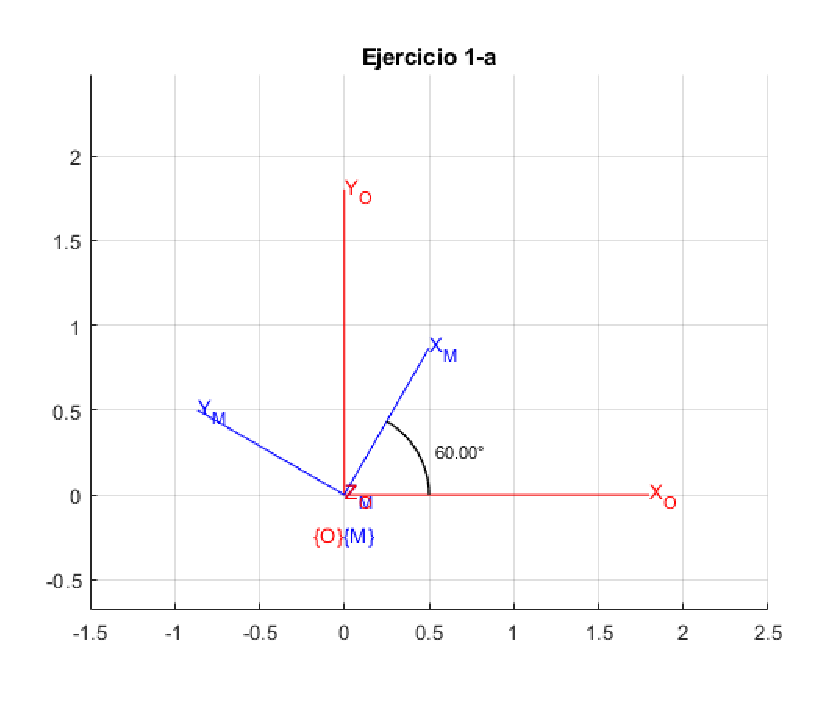
\includegraphics{1-Ejercicio_1_a.pdf}}
%    \end{adjustbox}
%    \caption{Sistema O y Sistema M superpuestos con indicación de ángulo de rotación.}
%\end{figure}


%\begin{table}[H]
%    \centering
%    \begin{tabular}{|c|c|c|c|c|c|}
%    \hline
%    Sistema & $\theta$  & $d$           & $a$    & $\alpha$ & $\sigma$ \\ \hline
%    1       & $q_1$     & $199.2$       & $200$  & 0        & 0        \\ \hline
%    2       & $q_2$     & $59.5$        & $250$  & 0        & 0        \\ \hline
%    3       & $0$       & $q_3$         & $0$    & 180°     & 1        \\ \hline
%    4       & $q_4$     & $37.5$        & $0$    & 0        & 0        \\ \hline
%    \end{tabular}
%    \caption{Parámetros DH alternativos.}
%    \label{parametros DH2}
%\end{table}

\end{document}